\documentclass[11pt]{article}

\usepackage{amsmath,amssymb, a4, verbatim}
\usepackage[german]{babel}
%\usepackage[latin1]{inputenc}
\usepackage[utf8]{inputenc} % üöäß
\usepackage{listings} % für inline codelistings
\lstset{%
	basicstyle=\ttfamily,  % the size of the fonts 
	columns=fixed, % anything else is horrifying
	showspaces=false,       % show spaces using underscores?
	showstringspaces=false, % underline spaces within strings?
	showtabs=false,% show tabs within strings?
	xleftmargin=1.5em,      % left margin space
}
\lstdefinestyle{inline}{basicstyle=\ttfamily}
\newcommand{\listline}[1]{\lstinline[style=inline]!#1!}


\usepackage{caption}
\newcommand{\tinycaption}[1]{\captionsetup{labelformat=empty}\caption{#1}}

%\usepackage{color}
%\usepackage{epsfig} % eps
\usepackage{graphicx} % eps
%\usepackage[shortcuts]{extdash}
%\usepackage{dsfont}
%\usepackage{epstopdf} % eps
%\usepackage[pdf]{pstricks} % eps
%\usepackage{auto-pst-pdf}
\usepackage{mathtools}
\usepackage{dsfont} % $ \mathds{1} $
\usepackage{icomma}
\usepackage{tikz}
%\usepackage{pgfplots}
%\pgfplotsset{compat=1.8}
\usepackage[bottom]{footmisc} % put footnotes at the bottom of page
\usepackage{nicefrac} % für brüche die aussehen wie prozentzeichen
% \usepackage{ps2pdf}
\usetikzlibrary{automata,positioning}

\usepackage{algorithmicx}
\usepackage{algpseudocode}
\usepackage{algorithm}

\usepackage{multicol}
\usepackage{wrapfig} % make stuff float
\usepackage{placeins} % stop stuff from floating
\usepackage{seqsplit} % very long numbers
\usepackage{framed} % begin{framed}

%  Headings and Footings :
\usepackage{fancyhdr}
\headheight15pt
\lhead{Anwendungsprogrammierung \ueberschrift} % TODO

\chead{}
\rhead{\thepage}
\renewcommand{\headrulewidth}{.4pt}

\lfoot{\today}
\cfoot{}
\rfoot{Name...} %TODO, würde ich erst am ende eintragen und generieren vorm abschicken, muss ja nicht bei github rumhängen
\renewcommand{\footrulewidth}{.4pt}

%----------------------------------------------------------------


\textwidth17.5cm % 16.5cm
\textheight23cm
\oddsidemargin0.cm
\evensidemargin0.cm
\voffset-1.5cm % move page up
\hoffset-0.5cm % move page to the left

\parindent0cm

\newcommand{\R}{{\mathbb R}}
\newcommand{\C}{{\mathbb C}}
\newcommand{\1}{{\mathds{1}}}
\newcommand{\abs}[1]{\lvert#1\rvert}
\newcommand{\norm}[1]{\left\lVert#1\right\rVert}
\newcommand{\xt}{\tilde{x}}
\newcommand{\dotleq}{\dot{\leq}}
\newcommand{\m}{\hphantom{-}}

\newcommand{\dashfill}[1]{\vspace{11pt}\def\dashfill{\cleaders\hbox{#1}\hfill}\hbox to \hsize{\dashfill\hfil}\vspace{11pt}}
\newcommand{\scdot}{\!\cdot\!}

\newcommand{\sig}{\text{signum}}
\newcommand{\rot}{}

% ------------------  edit Ueberschrift ---------------------
\newcommand{\ueberschrift}{Dokumentation} % TODO


\usepackage{varwidth}
\newcommand{\umrandet}[1]{\pbox{\textwidth}{\boxed{\text{#1}}}}

\newcommand{\aGreatFramedBox}[1]{\fbox{\begin{varwidth}{\textwidth}#1\end{varwidth}}\ignorespacesafterend}
\newcommand{\umramt}[1]{\begin{minipage}{\widthof{\aGreatFramedBox{#1}}}\aGreatFramedBox{#1}\ignorespacesafterend\end{minipage}\ignorespacesafterend}

\usepackage{pgf-umlcd}
\renewcommand{\umltextcolor}{black}
\renewcommand{\umldrawcolor}{gray}
\renewcommand{\umlfillcolor}{white}
% variables to tweak appearance of uml stuff
\newcommand{\umlScale}{0.9}
\newcommand{\umlScaleSpielController}{0.6}
\newcommand{\umlWidth}{.74\linewidth}
\newcommand{\imagewidth}{.8\linewidth}
% -----------------------------------------------------------
\begin{document}
	\pagestyle{fancy}
	
	\section*{Beschreibung des Programms aus Sicht der Anwender:}
	
	Das Programm bietet die Möglichkeit, mehrere Versionen des Spiels Gomoku bzw. 5 Gewinnt zu spielen.
	Dabei ist dem Spieler überlassen, ob er gegen den Computer, einen realen Gegner oder die künstliche Intelligenz gegen sich selbst spielen lassen möchte.
	Zusätzlich kann noch entschieden werden, wie viele in einer Reihe zum Sieg benötigt werden, 
	ob in der Mitte des Bretts begonnen werden soll und ob nur Anlegen an einen anderen Stein erlaubt ist.
	Die Brettgröße ist auch flexibel wählbar.
	
	\subsection*{Es sind folgende Spielregeln zu beachten:}
	Das klassische Gomoku wird auf einem $19 \times 19$ Brett gespielt.
	Dabei legt jeder Spieler abwechselnd einen Stein seiner Farbe auf das Brett.
	Die Steine dürfen nicht mehr bewegt werden, nachdem sie gesetzt wurden. Jeder versucht eine gerade, ununterbrochene Reihe aus 5 Spielsteinen zu legen.
	Die Reihe kann waagerecht, senkrecht oder diagonal verlaufen. 
	
	Gleichzeitig muss jeder Spieler verhindern, dass der andere Spieler dieses Ziel vor ihm erreicht.
	Das Spiel ist beendet, wenn ein Spieler 5 Steine in einer ununterbrochenen Reihe gelegt hat. 
	Die Spielregeln für alle anderen Versionen sind analog, es ändert sich nur die Brettgröße und die Anzahl Steine in einer Reihe, die zum Sieg benötigt werden. 
	
	
	\section*{Bedienungsanleitung}
	
	\section{Spiel Starten}
	Beim Starten des Programms erscheint folgende Oberfläche
	
	\begin{figure}[H]
		\centering
		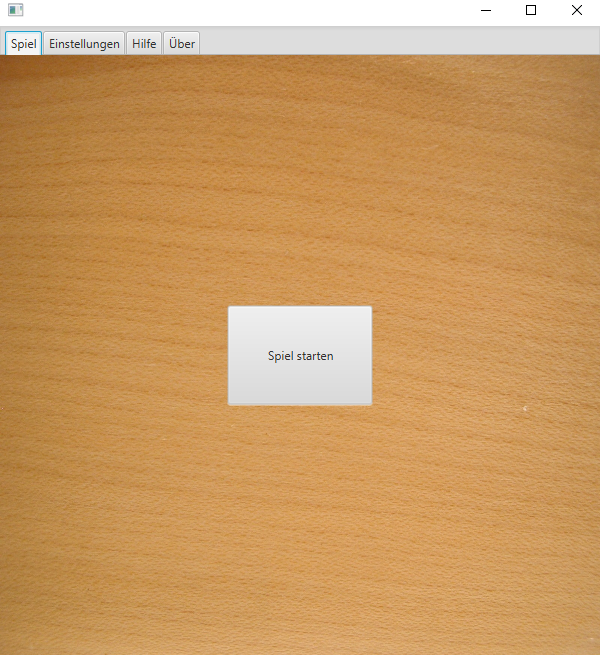
\includegraphics[width=\imagewidth]{starten.png}
		\caption{Aussehen nach Programmstart}
		\label{starten}
	\end{figure}
	
	Startet man nun das Spiel, indem man auf den \textit{Spiel starten} Button drückt, so werden die Standardeinstellungen geladen.
	Das heißt die AI spielt gegen sich selbst auf einem $19 \times 19$ Brett. 
	
	
	\section{Einstellungen ändern}
	Möchte man mit anderen Einstellungen spielen, so hat man die Möglichkeit diese zu ändern, indem man auf den \textit{Einstellungen Tab} wechselt. 
	
	\begin{figure}[H]
		\centering
		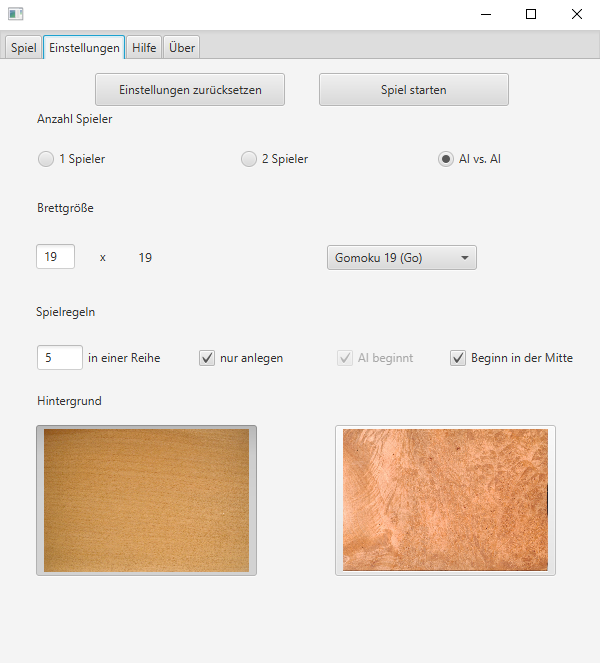
\includegraphics[width=\imagewidth]{einstellungen.png}
		\caption{Einstellungen Tab}
		\label{einstellungen}
	\end{figure}
	
	Die Anzahl der Spieler lässt sich einfach anklicken.
	Die gewünschte Brettgröße kann man eintippen, oder man entscheidet sich für eine der klassischen Varianten, auswählbar aus der Combo Box.
	Zur Auswahl stehen dabei Gomoku 19, 17 und 15 und Tic Tac Toe.
	Die Anzahl Steine in einer Reihe lassen sich auch einfach eintippen, die restlichen Einstellungen kann man auch beliebig an- bzw. wegklicken.
	Das Hintergrundbild ist auch veränderbar, zur Auswahl stehen die beiden unten abgebildetem Bilder, welche man nur anklicken braucht.
	
	Ist man mit seinen Einstellungen zufrieden, so klickt man auf den \textit{Spiel Starten} Button oben rechts.
	Dann wird automatisch zum \textit{Spiel} Tab gewechselt und man kann mit dem Spielen beginnen.
	
	Möchte man die Einstellungen wieder auf die Standardeinstellungen zurücksetzen, so braucht man nur den Button \textit{Einstellungen zurücksetzen} oben links zu klicken. 
	Zu beachten ist auch, dass sich die Einstellungen nicht ändern lassen, solange ein aktuelles Spiel noch läuft (s. nächster Abschnitt).
	
	\section{Spiel abbrechen und neues Spiel starten}
	
	Möchte man ein aktuell laufendes Spiel abbrechen, so klicke man den Button \textit{Neues Spiel} oben rechts.
	
	\begin{figure}[H]
		\centering
		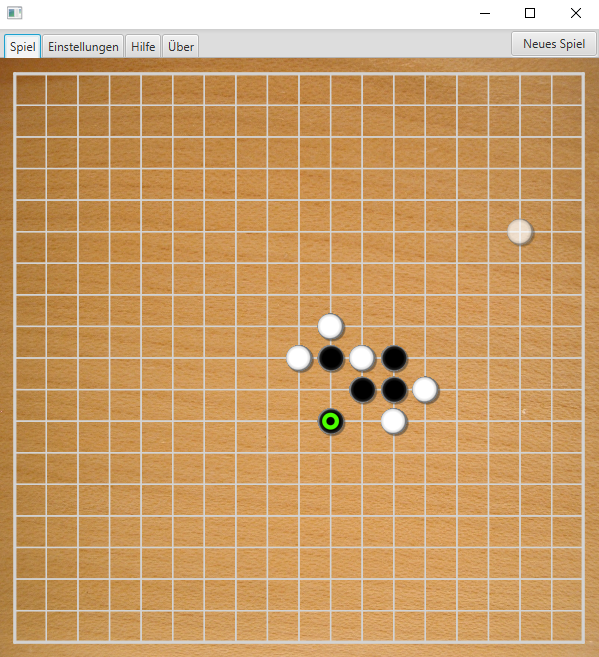
\includegraphics[width=\imagewidth]{spiel.png}
		\caption{Laufendes Spiel}
		\label{spiel}
	\end{figure}
	
	Hierbei ist zu beachten, dass dann allerdings der gesamte Spielfortschritt verloren gehen würde, wobei der Spieler auch eine Warnung erhält. 
	
	\begin{figure}[H]
		\centering
		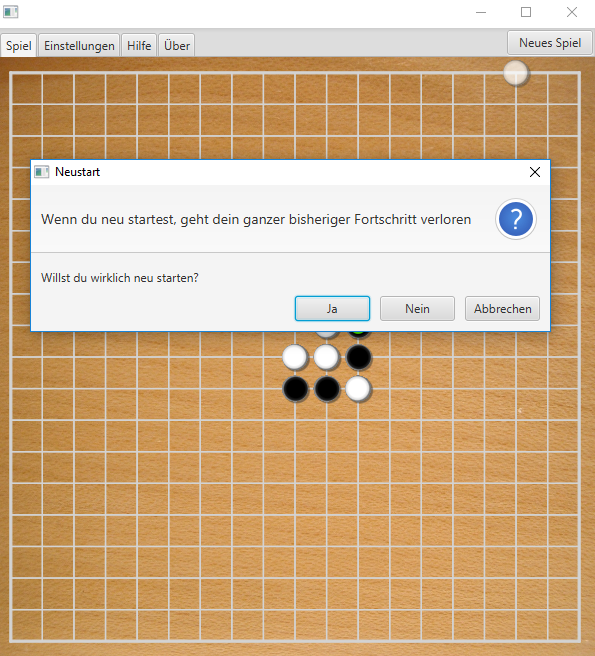
\includegraphics[width=\imagewidth]{warnung.png}
		\caption{Warnung vor Neustart}
		\label{warnung}
	\end{figure}
	
	Klickt man nun auf \textit{Ja}, hat man wieder die Möglichkeit, die Einstellungen zu ändern oder man startet ein neues Spiel mit den selben Einstellungen. 
	
	\section{AI gegen AI}
	
	Bei der Version AI gegen AI hat man noch zusätzliche Optionen. 
	
	Das Spiel lässt sich jederzeit pausieren, indem man auf den \textit{Pause/Play} Button drückt (links neben \textit{Neues Spiel}).
	Zudem lässt sich die Schnelligkeit der Züge beeinflussen anhand des Reglers links daneben. 
	
	\begin{figure}[H]
		\centering
		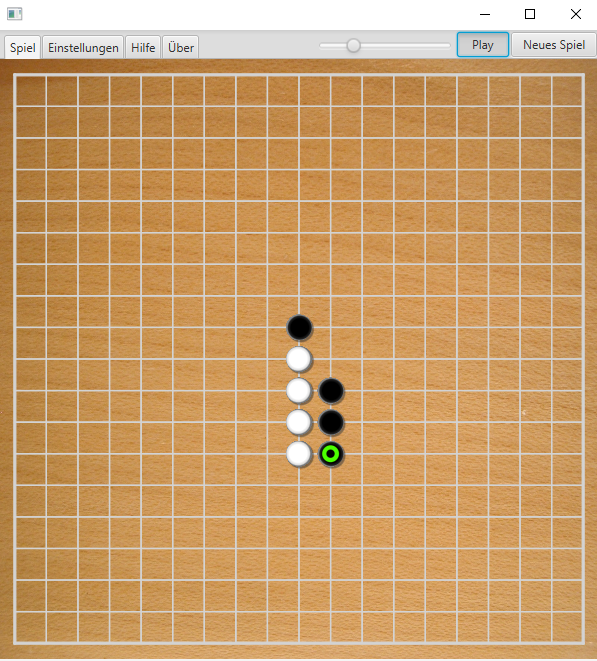
\includegraphics[width=\imagewidth]{ai.png}
		\caption{AI spielt gegen AI}
		\label{ai}
	\end{figure}
	
	\section{Spielzug machen}
	
	Der Stein des jeweiligen Spielers, der gerade an der Reihe ist, erscheint an dem Mauszeiger und bewegt sich mit, wenn die Maus verschoben wird
	Möchte man einen Stein irgendwo platzieren, so braucht man nur auf die jeweilige Stelle im Brett zu klicken.
	Der Stein wird dann dort abgelegt (solange diese Position legal ist, es also möglich ist an dieser Position zu spielen) und der Gegner ist an der Reihe. 

	\section{Gewinner}
	Sollte ein Spieler gewinnen, erscheint folgende Meldung. 

	\begin{figure}[H]
		\centering
		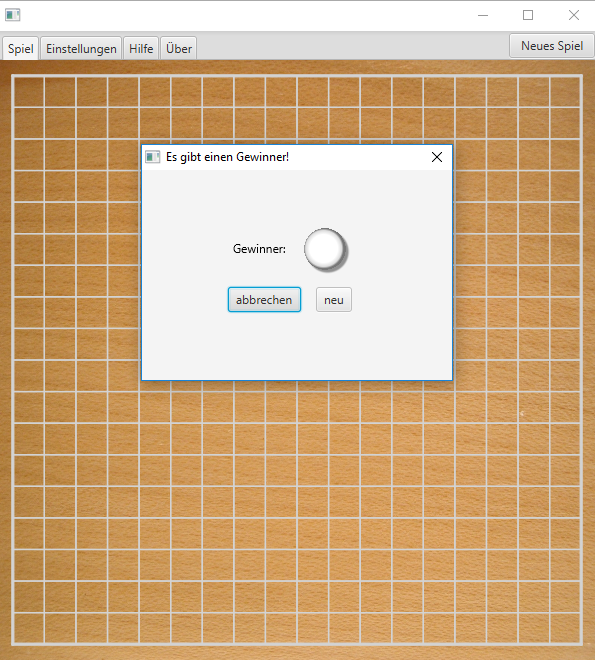
\includegraphics[width=\imagewidth]{gewinner.png}
		\caption{Meldung bei Gewinner}
		\label{gewinner}
	\end{figure}

	Hier hat man dann die Möglichkeit, das Spiel neu zu starten, indem man auf \textit{neu} klickt.
	Oder man klickt auf \textit{abbrechen}, um womöglich den Spielverlauf zu analysieren. 
	
	\section{Hilfe und Über}
	Die Spielanleitung ist im Tab \textit{Hilfe} nachzulesen und Informationen über Programm und Autor lassen sich im Tab \textit{Über} nachschauen. 
	
	\pagebreak
	
	Beschreibung des Programms aus Sicht der Programmierer
	
	Model
	
	Im Model befinden sich die folgenden Klassen:
	
	\begin{center}
		\begin{tabular}{r l}
			\lstinline|Brett| & zur Speicherung eines Spielbrettes \\
			\lstinline|Options| & speichert die Optionen als ein Paar zweier Objekte vom Typ \lstinline|String| und \lstinline|Object| \\
			\lstinline|SpielAI| & generiert die AI \\
			\lstinline|SpielStein| & zur Speicherung eines Spielsteins
		\end{tabular}
	\end{center}
	
	\begin{tikzpicture}[thick, scale=\umlScale, every node/.style={scale=\umlScale}]
		%\begin{package}{application}	
			%\begin{package}{model}
				\begin{class}[text width=\umlWidth]{Brett}{0, 0}
					\attribute{$-$ \_dim : int}
					\attribute{$-$ \_spieler : int}
					\attribute{$-$ \_brett : SpielStein[ ][ ]}
					\attribute{$-$ \_gitterVert : List$<$Line$>$}
					\attribute{$-$ \_gitterHorz : List$<$Line$>$}
					\attribute{$-$ \_gitter : List$<$Line$>$}
					\attribute{$-$ \_SpielZuege : List$<$SpielZug$>$} 
					\attribute{$-$ \_gitterWeite : double}
					\attribute{$-$ \_randX : double}
					\attribute{$-$ \_randY : double} 
					\attribute{$-$ \_CheckAdjacent : boolean}
					\operation{+ Brett(dim : int, x : double, y : double)} 
					\operation{+ redrawGitter(x : double, y : double) : void}
					\operation{+ roundCoord(x : double, y : double) : double[ ]}
					\operation{+ steinAt(int x, int y) : SpielStein}
					\operation{+ steinAt(double x, double y) : SpielStein}
					\operation{$-$ steinSet(int x, int y, SpielStein s) : boolean}
					\operation{+ makeMove(SpielZug zug) : boolean}
					
					\operation{+ printMoves() : void}
					\operation{+ getNextMoveColour() : int}
					\operation{+ List$<$SpielZug$>$ getSpielZuege() : final}
					\operation{+ getDim() : int}
					\operation{+ getGitter() : List$<$Line$>$}
					\operation{+ getGitterWeite() : double}
					\operation{+ getRandX() : double}
					\operation{+ getRandY() : double}
					\operation{+ getSpieler() : final int}
					\operation{+ getBrett() : final SpielStein[ ][ ]}
				\end{class}
				\begin{class}[text width=\umlWidth]{+ static SpielZug}{0, -14.5}
					\attribute{+ x, y : int}
					\attribute{+ stein:SpielStein}
					\attribute{+ iView:ImageView}
					\operation{+ SpielZug(x:int, y:int, stein:SpielStein, iView:ImageView)}
					\operation{+ toString():String}
				\end{class}
			%\end{package}%model
		%\end{package}%application
	\end{tikzpicture}
	
	\begin{tikzpicture}[thick, scale=\umlScale, every node/.style={scale=\umlScale}]
		%\begin{package}{application}	
			%\begin{package}{model}
				\begin{class}[text width=\umlWidth]{Options}{0, 0}
					\attribute{$-$ \_menge : HashSet$<$Tupel$>$}
					\operation{+ Options()}
					\operation{+ setOption(name : String , objekt : Object) : void}
					\operation{+ getOption(name : String) : Object}
					\operation{+ printOption(name : String) : void}
					\operation{+ toString() : String}
				\end{class}
				\begin{class}[text width=\umlWidth]{-Tupel}{0, -4.0}
					\attribute{+ name : String}
					\attribute{+ objekt : Object}
					\operation{+ Tupel(name : String, objekt : Object)}
					\operation{+ hashCode() : int}
					\operation{+ equals(Object obj) : boolean}
					\operation{$-$ getOuterType() : Options}
					\operation{+ toString() : String}
				\end{class}
			%\end{package}%model
		%\end{package}%application
	\end{tikzpicture}
	
	\begin{tikzpicture}[thick, scale=\umlScale, every node/.style={scale=\umlScale}]
		%\begin{package}{application}
			%\begin{package}{model}
				\begin{class}[text width=\umlWidth]{SpielAI}{0, 0}
					\attribute{$-$ \_brett : Brett}
					\attribute{$-$ \_possibleMoves : ArrayList$<$LinkedHashSet$<$Savegame$>>$}
					\operation{+ SpielAI(brett : Brett) }
					\operation{+ generateNextMoves() : void}
					\operation{+ updateMoves() : void}
					\operation{+ getBestMoves() : Integer[ ][ ]}		
					\operation{+ addDoubleArray(a : Double[ ][ ], b : Double[ ][ ]) : static Double[ ][ ] }
					\operation{+ multDoubleArray(a : Double[ ][ ], f : double) : static void }
					\operation{+ twoDeepCloneDouble(a : Double[ ][ ]) : static Double[ ][ ] }
					\operation{+ printDoubleArray(a : Double[ ][ ]) : static void }
				\end{class}
				\begin{class}[text width=\umlWidth]{Savegame}{0, -6}
					\attribute{$-$ moveNr : int}
					\attribute{$-$ steine : int[ ][ ]}
					\attribute{$-$ spielerAnz : int}
					\attribute{$-$ dim : int}
					\attribute{$-$ nextMove : int[ ]}
					\operation{+ Savegame(brett : Brett)}
					\operation{+ generateNextMoves() : LinkedHashSet$<$Savegame$>$}
					\operation{+ generateHeuristic() : Double[ ][ ]}
					\operation{+ hashCode() : int}
					\operation{+ toString() : String}
					\operation{+ equals(obj : Object) : boolean}
				\end{class}
			%\end{package}%model
		%\end{package}%application
	\end{tikzpicture}
	
	\begin{tikzpicture}[thick, scale=\umlScale, every node/.style={scale=\umlScale}]
		%\begin{package}{application}
			%\begin{package}{model}{0,-10}
				\begin{class}[text width=\umlWidth]{SpielStein}{0, 0}
					\attribute{$-$ farbe : int}
					\attribute{$-$ img : Image}
					\attribute{$-$ blackStone : static Image}
					\attribute{$-$ whiteStone : static Image}
					
					\operation{+ getColor() : final int}
					\operation{+ getImage() : final Image}
				\end{class}
			%\end{package}%model
		%\end{package}%application
	\end{tikzpicture}
	
	(Hier noch UML Diagramme einfügen und Algorithmen in Pseudo Code)
	
	
	View
	
	(Hier Scene Graph einfügen)
	
	Controller
	
	Der Spielcontroller ist zuständig für das gesamte Spiellayout.
	Zusätzlich gibt es noch den \lstinline|GewinnerController| für das \lstinline|GewinnerLayout|,
	welches immer dann erscheint, sobald ein Spieler gewonnen hat bzw. unentschieden gespielt wurde. 
	
	(Hier UML-Diagramme einfügen bzw. Algorithmen )
	
	
	
	
	
	
	
	
	
	
	
	
	
	
	
	
	
	
	
	
	
	
	
	
	
	
	
	
	
	
	
	
	\begin{tikzpicture}[thick, scale=\umlScale, every node/.style={scale=\umlScale}]
		%\begin{package}{application}
			%\begin{package}{view}
				\begin{class}[text width=\umlWidth]{GewinnerController}{0, 0}
					\attribute{$-$ gewinnerPane : AnchorPane}
					\attribute{$-$ abbrechenButton : Button}
					\attribute{$-$ neuButton : Button}
					\attribute{$-$ gewinneriView :ImageView}
					\attribute{$-$ gewinnerText : Text}				
					\attribute{$-$ spielController : SpielController}
					\attribute{$-$ gewinnerStage : Stage}
					\operation{+ handleAbbrechenButton(event : ActionEvent) : void}
					\operation{+ handleNeuButton(event : ActionEvent) : void}
					\operation{+ setGewinnerImage(image Image) : void}		
					\operation{+ setDialogStage(gewinnerStage : Stage) : void}
					\operation{+ setGewinnerText(s : String) : void}
					\operation{+ setDialogSpielController(spielController : SpielController):void}
				\end{class}
			%\end{package}%view
		%\end{package}%application
	\end{tikzpicture}

	\begin{tikzpicture}[thick, scale=\umlScale, every node/.style={scale=\umlScale}]
		%\begin{package}{application}
			\begin{class}[text width=\umlWidth]{Main}{0, 0}
				\attribute{+ optionen : static Options}
				\attribute{+ primaryStage : static Stage}
				\operation{+ start(primaryStage : Stage) : void}
				\operation{+ main(args : String[]) : static void}
			\end{class}
		%\end{package}%application
	\end{tikzpicture}
	
	\begin{tikzpicture}[thick, scale=\umlScaleSpielController, every node/.style={scale=\umlScaleSpielController}]
		%\begin{package}{application}
			%\begin{package}{view}
				\begin{class}[text width=\umlWidth]{SpielController}{0, 0}
					\attribute{$-$ mitteBeginnCheckBox : CheckBox }
					\attribute{$-$ backgroundImage : ImageView }
					\attribute{$-$ tabPaneSwitch : TabPane }
					\attribute{$-$ ueberTab : Tab }
					\attribute{$-$ anlegenCheckBox : CheckBox }
					\attribute{$-$ brettGroesseLabel : Label }
					\attribute{$-$ einstellungenAnchorPane : AnchorPane }
					\attribute{$-$ gameAnchorPane : AnchorPane }
					\attribute{$-$ aiCheckBox : CheckBox }
					\attribute{$-$ helpTab : Tab }
					\attribute{$-$ gameTab : Tab }
					\attribute{$-$ brettGroesseTextField : TextField }
					\attribute{$-$ zweiSpielerButton : RadioButton }
					\attribute{$-$ stoneImage : ImageView }
					\attribute{$-$ brettGroesseBox : ComboBox$<$String$>$ }
					\attribute{$-$ bild2Button : ToggleButton }
					\attribute{$-$ einstellungenTab : Tab }
					\attribute{$-$ anzahlReiheTextField : TextField }
					\attribute{$-$ bild1Button : ToggleButton }
					\attribute{$-$ einSpielerButton : RadioButton }
					\attribute{$-$ aiButton : RadioButton }
					\attribute{$-$ hilfeText : TextArea }
					\attribute{$-$ uberText : TextArea }
					\attribute{$-$ neuButton : Button }
					\attribute{$-$ spielStartenButton : Button }
					\attribute{$-$ startButton : Button }
					\attribute{$-$ newGameButton : Button }
					\attribute{$-$ pauseGameButton : ToggleButton }
					\attribute{$-$ zuruecksetzenButton : Button }
					\attribute{$-$ wrapAnchorPane : AnchorPane }
					\attribute{$-$ aiSpeedSlider : Slider }
					\attribute{$-$ radioButtonGroup : final ToggleGroup }
					\attribute{$-$ bildGroup : final ToggleGroup }
					\attribute{$-$ choiceBoxOptions : ObservableList$<$String$>$ } 
					\attribute{$-$ spielbrett : Brett }
					\attribute{$-$ gameDone : boolean }
					\attribute{$-$ s : SpielStein }
					\attribute{$-$ currWidth, currHeight : double }
					\attribute{$-$ lastPlayed : ImageView }
					\attribute{$-$ winningStone : List$<$ImageView$>$ }
					\attribute{$-$ gegner : SpielAI }
					\attribute{$-$ lastTime : static long }
					\attribute{$-$ aiPaused : boolean }
					\attribute{$-$ zweiAiTimer : AnimationTimer }
					 
					\operation{ $-$ initialize() : void }
					\operation{ $-$ standardEinstellungen() : void }
					\operation{ + bildeBrett() : void }
					\operation{ $-$ handleSpielerAnzahlButton(ActionEvent event) : void }
					\operation{ $-$ handleBrettGroesseBox(ActionEvent event) : void }
					\operation{ $-$ handleBrettGroesseFeld(ActionEvent event) : void }
					\operation{ $-$ handleSpielregeln(ActionEvent event) : void }
					\operation{ $-$ handleBackground(ActionEvent event) : void }
					\operation{ + neustart() : void }
					\operation{ $-$ handleSpielStartenButton() : void }
					\operation{ $-$ handleZuruecksetzenButton(ActionEvent event) : void }
					\operation{ $-$ handleStartButton() : void }
					\operation{ $-$ disable() : void }
					\operation{ $-$ enable() : void }
					\operation{ $-$ handleNewGameButton() : void }
					\operation{ $-$ handlePauseGameButton(ActionEvent event) : void }
					\operation{ $-$ handleMouseMoved(MouseEvent event) : void }
					\operation{ $-$ handleSizeChanged() : void }
					\operation{ $-$ handleSizeChanged(boolean forceIt) : void }
					\operation{ $-$ updatePlayMarkers() : void }
					\operation{ $-$ handleDragDetected(MouseEvent event) : void }
					\operation{ $-$ handleMouseClicked(int x, int y) : void }
					\operation{ $-$ handleMouseClicked(MouseEvent event) : void }
					\operation{ $-$ letAImakeMove() : void }
					\operation{ $-$ handleGewinner() : boolean }
					\operation{ $-$ handleGewinner(boolean unentschieden) : boolean }
					\operation{ $-$ checkIfGewinner() : boolean }
					\operation{ $-$ handleKeyPressed(KeyEvent event) : void }
					\operation{ $-$ handleKeyReleased(KeyEvent event) : void }
				\end{class}
			%\end{package}%model
		%\end{package}%application
	\end{tikzpicture}
	

		

	
	\begin{wrapfigure}{L}{\textwidth}
		getBestMoves():\\
		\umramt{\begin{varwidth}{\textwidth}
			\begin{algorithmic}[1]
				\State $h\leftarrow$ generateHeuristic()
				\State $max \leftarrow-\infty$
				\State $n\leftarrow 0$
				\For{$i \in \{0, dim(h)\} $}
					\For{$j \in \{0, dim(h)\} $}
						\If{$max < h_{i, j}$}
							\State $max \leftarrow h_{i, j}$
							\State $n\leftarrow 1$
						\ElsIf{$max=h_{i, j}$}
							\State $n++$
						\EndIf
					\EndFor
				\EndFor
				\State $erg :\in {\mathbb{N}}^{\text{n}\times 2}$
				\For{$i \in \{0, dim(h)\} $}
					\For{$j \in \{0, dim(h)\} $}
						\If{ $max = h_{i, j}$ }
							\State 	$n \leftarrow n-1$
							\State 	$erg_{n, 0}\leftarrow i$
							\State 	$erg_{n, 1}\leftarrow j$
						\EndIf
					\EndFor
				\EndFor
				\State\Return erg
			\end{algorithmic}
		\end{varwidth}}%
	\end{wrapfigure}
	
\end{document}














































